\gls{descan} is an R \cite{Ihaka1996} tool developed for detecting open chromatin regions signal in order to facilitate the differential enrichment of genomic regions between two or more biological conditions.

The package has been implemented using Bioconductor \cite{Gentleman2004} data structures and methods, and it is available through the Bioconductor repository since version 3.7.

The tool is organized into three main steps. 
A peak caller, which is a standard moving scan window that compares the reads coverage signal within a sliding window to the signal in a larger region outside the window. It uses a Maximum Likelihood Estimator of a Poisson Distribution, providing a final score for each detected peak.

The filtering and alignment steps are aimed to determine if a peak is a "true peak" on the basis of its replicability in other samples. 
These steps are grouped in a single procedure and are based on a double user-defined threshold, one on the peaks scores and one on the number of samples.

The third step produces a count matrix where each column represents a sample and each row a peak. The value of each cell represents the number of reads for the peak in the sample.

The produced count matrix, as illustrated in figure \ref{fig:descan2flow}, is useful both for doing differential enrichment between multiple conditions and for integrating the epigenomic data with other -omic data types.


\begin{figure}[H]
\centering
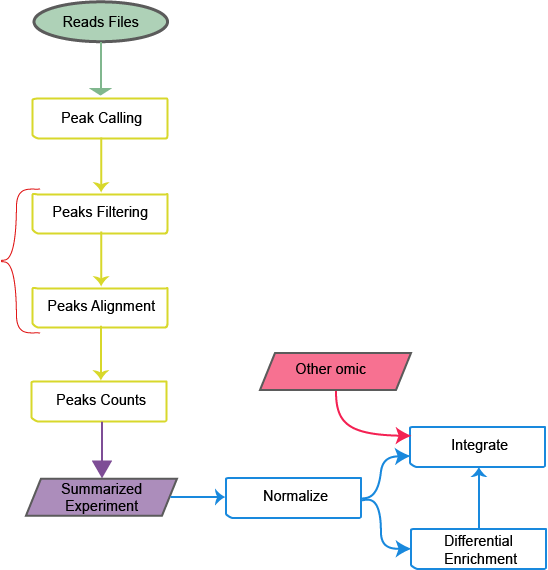
\includegraphics[width=8cm, keepaspectratio]{img/descan2/flow.png}
\caption[DEScan2 workflow]{A differential enrichement flow representation. \gls{descan} steps are highlighed in yellow.}
\label{fig:descan2flow}
\end{figure}

